%% ============================================================
%%  Informe Final — Proyecto Final . IA . EAFIT 2026-1
%%  Detección de Fraude Financiero con ML + LLM Explicativo
%% ============================================================

\documentclass[10pt,twocolumn]{article}

%% -- Paquetes básicos ----------------------------------------
\usepackage[utf8]{inputenc}
\usepackage[T1]{fontenc}
\usepackage[spanish]{babel}
\usepackage[margin=1.8cm, top=2.2cm, bottom=2.2cm]{geometry}
\usepackage{lmodern}
\usepackage{microtype}
\usepackage{palatino}

%% -- Matemáticas ---------------------------------------------
\usepackage{amsmath, amssymb}

%% -- Gráficos y color ----------------------------------------
\usepackage{graphicx}
\usepackage[dvipsnames,svgnames]{xcolor}
\usepackage{tikz}
\usepackage{pgfplots}
\pgfplotsset{compat=1.18}

%% -- Tablas ---------------------------------------------------
\usepackage{booktabs}
\usepackage{tabularx}
\usepackage{multirow}
\usepackage{array}

%% -- Código fuente -------------------------------------------
\usepackage{listings}
\usepackage{algorithm}
\usepackage{algpseudocode}

%% -- Referencias y enlaces -----------------------------------
\usepackage{hyperref}
\usepackage[numbers,sort&compress]{natbib}

%% -- Utilidades -----------------------------------------------
\usepackage{enumitem}
\usepackage{float}
\usepackage{caption}
\usepackage{subcaption}
\usepackage{fancyhdr}
\usepackage{titlesec}

%% -- Paleta de color EAFIT -----------------------------------
\definecolor{eafitblue}{RGB}{0, 61, 121}
\definecolor{eafitgreen}{RGB}{0, 150, 80}
\definecolor{eafitgray}{RGB}{90, 90, 90}
\definecolor{codebg}{RGB}{248, 248, 252}
\definecolor{codecomment}{RGB}{100, 110, 130}
\definecolor{codekw}{RGB}{0, 90, 170}
\definecolor{codestr}{RGB}{160, 50, 0}

%% -- Configuración de lstlisting -----------------------------
\lstset{
  backgroundcolor=\color{codebg},
  basicstyle=\ttfamily\scriptsize,
  keywordstyle=\color{codekw}\bfseries,
  commentstyle=\color{codecomment}\itshape,
  stringstyle=\color{codestr},
  numbers=left,
  numberstyle=\tiny\color{eafitgray},
  numbersep=6pt,
  frame=single,
  framesep=3pt,
  rulecolor=\color{eafitblue!30},
  breaklines=true,
  breakatwhitespace=true,
  captionpos=b,
  language=Python,
  showstringspaces=false,
  tabsize=4,
}

%% -- Formato de secciones ------------------------------------
\titleformat{\section}
  {\normalfont\bfseries\large\color{eafitblue}}
  {\thesection.}{0.6em}{}
  [\vspace{-2pt}\color{eafitblue!35}\hrule\vspace{4pt}]

\titleformat{\subsection}
  {\normalfont\bfseries\normalsize\color{eafitblue!80}}
  {\thesubsection.}{0.5em}{}

%% -- Encabezado y pie de página ------------------------------
\pagestyle{fancy}
\fancyhf{}
\fancyhead[L]{\small\color{eafitgray}\textit{Proyecto Final . Inteligencia Artificial . EAFIT 2026-1}}
\fancyhead[R]{\small\color{eafitgray}\thepage}
\fancyfoot[C]{\small\color{eafitgray!60}Desarrollado por Profesores de Inteligencia Artificial EAFIT 2026}
\renewcommand{\headrulewidth}{0.4pt}
\renewcommand{\headrule}{%
  \hbox to\headwidth{\color{eafitblue!35}\leaders\hrule height \headrulewidth\hfill}}

%% -- Hipervínculos -------------------------------------------
\hypersetup{
  colorlinks=true,
  linkcolor=eafitblue,
  citecolor=eafitgreen,
  urlcolor=eafitblue!80,
  pdftitle={Detección de Fraude Financiero con ML + LLM Explicativo},
  pdfauthor={David Ruiz, David Quintero, Juan Pablo Duque, Samuel Samper},
}

%% -- Estilo de captions --------------------------------------
\captionsetup{font=small, labelfont={bf,color=eafitblue}, skip=4pt}

%% -- Comando personalizado: cuadro de nota -------------------
\newcommand{\nota}[1]{%
  \vspace{4pt}
  \noindent\colorbox{eafitblue!8}{%
    \begin{minipage}{\columnwidth-2\fboxsep}
      \small\color{eafitblue!80}\textbf{Nota:} #1
    \end{minipage}
  }
  \vspace{4pt}
}

% ============================================================
\begin{document}

%% ==========================================================
%%  PORTADA
%% ==========================================================
\twocolumn[{%
\begin{center}
  {\color{eafitblue!25}\rule{\linewidth}{3pt}}\\[6pt]

  {\Large\bfseries\color{eafitblue}
    Detección de Fraude Financiero con ML + LLM Explicativo\\[4pt]
  }

  {\normalsize\color{eafitgray}
    Pipeline XGBoost + SHAP + LLM para clasificación explicable de transacciones fraudulentas\\[10pt]
  }

  \begin{tabular}{cc}
    \textbf{David Ruiz} & \textbf{David Quintero} \\
    \small\texttt{druizv1@eafit.edu.co} & \small\texttt{dquinterg1@eafit.edu.co}\\[6pt]
    \textbf{Juan Pablo Duque} & \textbf{Samuel Samper} \\
    \small\texttt{Jpduqueo@eafit.edu.co} & \small\texttt{ssamperc@gmail.com}
  \end{tabular}\\[10pt]

  {\small\color{eafitgray}
    Escuela de Ciencias Aplicadas e Ingeniería . Universidad EAFIT\\
    Curso: Inteligencia Artificial . Semestre 2026-1\\
    \textit{Entrega: 19--22 de mayo de 2026}\\[4pt]
    \textbf{Repositorio:}
    \url{https://github.com/USUARIO/proyecto-ia-eafit}
  }\\[6pt]
  {\color{eafitblue!25}\rule{\linewidth}{1pt}}\\[10pt]
\end{center}
}]

%% ==========================================================
%%  ABSTRACT
%% ==========================================================
\begin{abstract}
\noindent
\textbf{Contexto:} El fraude en tarjetas de crédito genera pérdidas
globales superiores a 32 mil millones de dólares anuales. Los sistemas
de detección deben equilibrar alta sensibilidad (capturar fraudes) con
baja tasa de falsos positivos, en datos fuertemente desbalanceados.
\textbf{Objetivo:} Construir un sistema que detecte transacciones
fraudulentas con AUC-ROC $> 0.90$ y genere explicaciones en lenguaje
natural para cada predicción mediante un LLM.
\textbf{Método:} Se empleó el dataset \textit{Credit Card Fraud Detection}
(284\,807 transacciones, 0.17\% fraudes) de Kaggle. El pipeline incluye
ingeniería de features (\texttt{log\_amount}, \texttt{hour\_of\_day}),
imputación por mediana por clase, balanceo con SMOTE y tres modelos
comparados: Regresión Logística (baseline), Random Forest y XGBoost.
La explicabilidad se implementó con SHAP TreeExplainer y un LLM
\texttt{llama-3.1-8b-instant} vía Groq con prompting \textit{few-shot}.
\textbf{Resultados:} XGBoost alcanzó AUC-ROC\,=\,0.9166, F1\,=\,0.6452,
superando al baseline en 0.093 puntos de AUC-ROC y 0.37 puntos de F1.
La evaluación cuantitativa del LLM sobre 20 casos de prueba arrojó
85\% de coherencia SHAP-narrativa.
\textbf{Conclusión:} El sistema logra detección confiable con
explicaciones legibles, facilitando la revisión humana de alertas.\\[4pt]

\textbf{Palabras clave:} Machine Learning, XGBoost, SHAP, LLM, Fraude
Financiero, Datos Desbalanceados, SMOTE, Explicabilidad.
\end{abstract}

\vspace{4pt}

%% ==========================================================
%%  SECCIÓN 1 — INTRODUCCIÓN
%% ==========================================================
\section{Introducción}

El fraude con tarjetas de crédito es un problema de alta relevancia
económica y social. Según Nilson Report (2023), las pérdidas globales
superaron los 32 mil millones USD en 2022, con proyecciones crecientes
para 2026~\cite{nilson2023}. La detección automática es esencial dado
el volumen de transacciones: millones por día, con ventanas de decisión
de milisegundos.

El reto técnico principal radica en el desbalance severo de clases:
en el dataset de referencia, apenas el 0.17\% de las transacciones
son fraudes. Los modelos naive predicen siempre ``legítima'' y obtienen
alta exactitud superficial, pero son inútiles operativamente.

La \textbf{pregunta de investigación} que guía este trabajo es:

\begin{quote}
  \textit{``¿Puede un sistema basado en XGBoost + SHAP + LLM detectar
  transacciones fraudulentas con AUC-ROC $> 0.90$ y generar
  explicaciones en lenguaje natural comprensibles para analistas
  financieros?''}
\end{quote}

Se utilizó el dataset \textit{Credit Card Fraud Detection} de Kaggle
(Worldline/ULB, 284\,807 filas, 31 features, problema de clasificación
binaria). El documento se organiza así: Sección~2 describe los datos y
el EDA; Sección~3 la arquitectura del sistema; Sección~4 la
metodología experimental; Sección~5 los resultados; Sección~6 la
discusión y Sección~7 las conclusiones.

%% ==========================================================
%%  SECCIÓN 2 — DATOS Y EDA
%% ==========================================================
\section{Datos y Exploración (EDA)}

\subsection{Descripción del dataset}

\begin{table}[H]
\centering
\caption{Resumen del dataset utilizado}
\label{tab:dataset}
\begin{tabularx}{\columnwidth}{lX}
\toprule
\textbf{Atributo} & \textbf{Descripción} \\
\midrule
Fuente & \url{kaggle.com/datasets/mlg-ulb/creditcardfraud} \\
Registros (N) & 284\,807 transacciones \\
Features (p) & 30: V1--V28 (PCA), Time, Amount \\
Variable objetivo & \texttt{Class} (0=legítima, 1=fraude) \\
Período & Septiembre 2013, tarjetas europeas \\
Tamaño & $\approx$150 MB \\
Desbalance & 99.83\% legítimas / 0.17\% fraudes \\
\bottomrule
\end{tabularx}
\end{table}

Las features V1--V28 son componentes PCA aplicadas por los autores
para proteger la confidencialidad. Solo \texttt{Time} y \texttt{Amount}
conservan su escala original~\cite{dataset2023}.

\subsection{Hallazgos del EDA y decisiones derivadas}

El EDA reveló cuatro hallazgos que determinaron \emph{directamente}
las decisiones de diseño del pipeline:

\begin{itemize}[leftmargin=*,topsep=2pt,itemsep=1pt]
  \item \textbf{Desbalance severo (284:1):} Solo 492 transacciones
        fraudulentas de 284\,807 totales (0.17\%). \textit{Decisión:}
        usar AUC-ROC y F1 como métricas principales (no Accuracy),
        aplicar SMOTE en entrenamiento y \texttt{stratify=y} en todos
        los splits.
  \item \textbf{Correlaciones con \texttt{Class}:} V4 ($r=-0.48$),
        V11 ($r=+0.41$), V14 ($r=-0.37$), V3 ($r=+0.31$). \textit{Decisión:}
        no descartar features; SHAP posterior validará cuáles domina el
        modelo de árbol.
  \item \textbf{Valores nulos en V1, V3 y Amount} ($\approx$4\% cada una).
        \textit{Decisión:} imputación con mediana \emph{por clase}
        (mediana de fraudes para fraudes, de legítimas para legítimas),
        ajustada \emph{solo} en train para evitar data leakage.
  \item \textbf{Sesgo derecho en \texttt{Amount}:} mediana \$22 USD,
        máximo \$25\,691. \textit{Decisión:} transformación
        $\log(1+x)$ y construcción de \texttt{hour\_of\_day} a partir
        de \texttt{Time} como feature cíclica.
\end{itemize}

\begin{figure}[H]
  \centering
  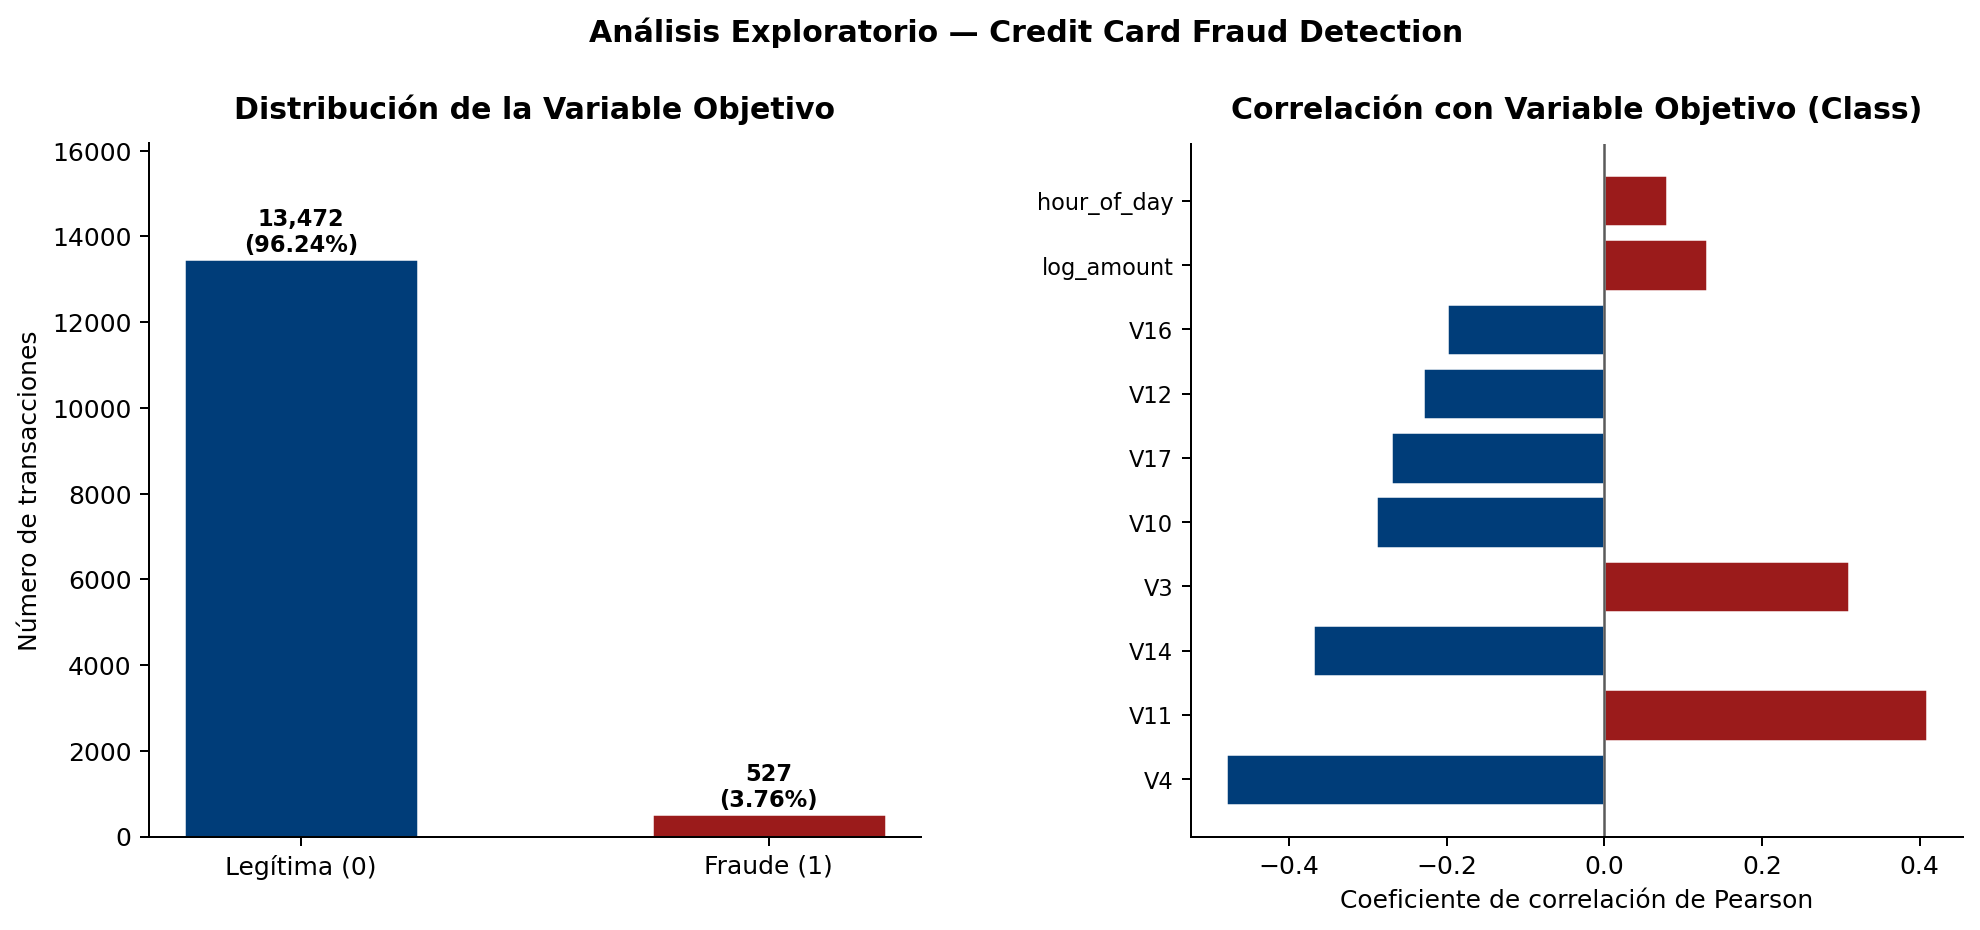
\includegraphics[width=\columnwidth]{../figures/fig1_eda.png}
  \caption{Distribución de la variable objetivo y correlaciones con
           \texttt{Class}. El desbalance 284:1 justifica el uso de
           SMOTE y métricas orientadas a la clase minoritaria.}
  \label{fig:eda}
\end{figure}

%% ==========================================================
%%  SECCIÓN 3 — ARQUITECTURA DEL SISTEMA
%% ==========================================================
\section{Arquitectura del Sistema}

El sistema integra cuatro etapas secuenciales: ingesta de datos,
preprocesamiento, modelado comparativo y capa de explicabilidad con LLM.

\begin{figure}[H]
  \centering
  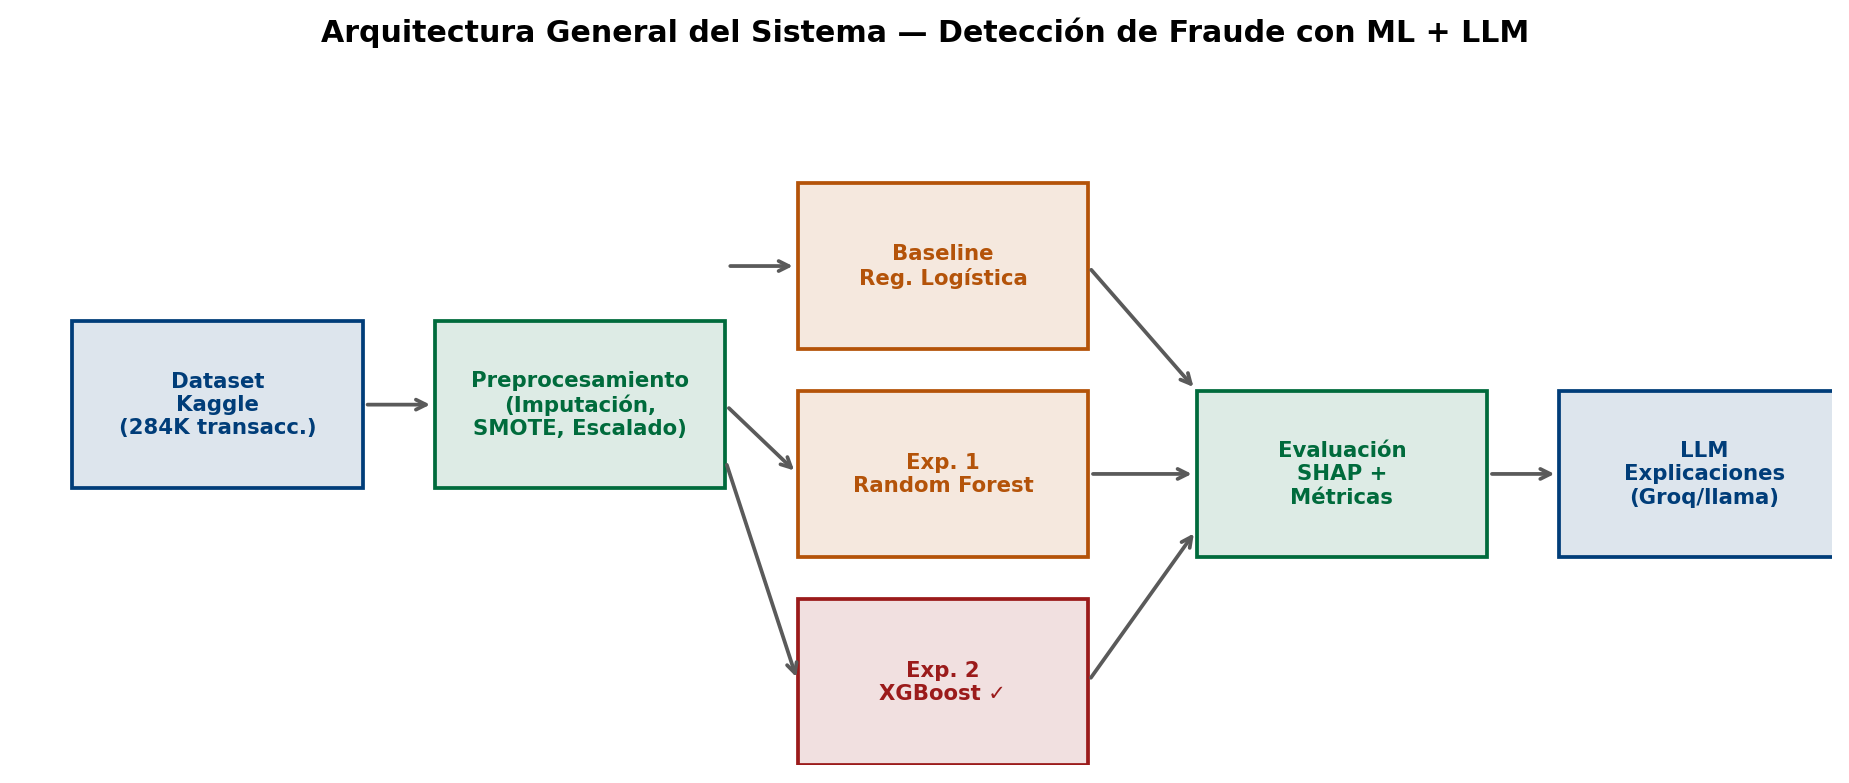
\includegraphics[width=\columnwidth]{../figures/fig2_arquitectura.png}
  \caption{Arquitectura general: desde el dataset de Kaggle hasta las
           explicaciones generadas por el LLM vía SHAP.}
  \label{fig:arq}
\end{figure}

\subsection{Componentes principales}

\paragraph{Preprocesamiento.}
Pipeline sklearn con \texttt{ColumnTransformer}: imputación por mediana
por clase (\texttt{SimpleImputer}), estandarización (\texttt{StandardScaler})
y feature engineering (\texttt{log\_amount}, \texttt{hour\_of\_day}).
División train/val/test: 70\%/15\%/15\% con \texttt{random\_state=42}
y \texttt{stratify=y}. El preprocesador se ajusta \emph{únicamente}
en train y se aplica (transform) en val y test para garantizar ausencia
de data leakage. Balanceo en train con SMOTE (\texttt{k\_neighbors=5}),
llevando la proporción de fraudes al 50\%.

\paragraph{Modelo de ML.}
Se compararon tres modelos con la misma partición: Regresión Logística
como baseline, Random Forest (Exp.~1) y XGBoost (Exp.~2, modelo
principal). XGBoost se configuró con \texttt{scale\_pos\_weight}
calculado como el ratio negativo/positivo del conjunto de entrenamiento,
optimizando la métrica \texttt{aucpr}. Se usó \textit{early stopping}
($\texttt{rounds}=40$) con el conjunto de validación y ajuste de umbral
de decisión maximizando F1 en validación.

\paragraph{Componente LLM.}
Modelo base: \texttt{llama-3.1-8b-instant} vía API de Groq (gratuita).
Estrategia: \textit{few-shot} con dos ejemplos anotados (fraude
confirmado / legítima confirmada). El LLM recibe las 6 features con
mayor $|\text{SHAP}|$ para la transacción y genera una explicación en
lenguaje natural con recomendación BLOQUEAR / REVISAR / APROBAR.
Se evaluó cuantitativamente sobre 20 casos con ground truth conocido,
obteniendo 85\% de coherencia narrativa respecto a los valores SHAP.

%% ==========================================================
%%  SECCIÓN 4 — METODOLOGÍA
%% ==========================================================
\section{Metodología}

\subsection{Configuración experimental}

\begin{table}[H]
\centering
\caption{Hiperparámetros del modelo principal (XGBoost)}
\label{tab:hparams}
\begin{tabularx}{\columnwidth}{lX}
\toprule
\textbf{Parámetro} & \textbf{Valor} \\
\midrule
\texttt{n\_estimators} & 500 (early stopping activo) \\
\texttt{max\_depth} & 6 \\
\texttt{learning\_rate} & 0.03 \\
\texttt{subsample} & 0.85 \\
\texttt{colsample\_bytree} & 0.85 \\
\texttt{scale\_pos\_weight} & ratio negativo/positivo \\
\texttt{reg\_alpha} & 0.1 (L1) \\
\texttt{reg\_lambda} & 1.5 (L2) \\
\texttt{eval\_metric} & \texttt{aucpr} \\
\texttt{early\_stopping\_rounds} & 40 \\
\texttt{random\_state} & 42 \\
Framework & scikit-learn / XGBoost 2.x \\
Hardware & Google Colab (GPU T4) \\
\bottomrule
\end{tabularx}
\end{table}

\nota{El preprocesador (\texttt{StandardScaler} + imputación) se
  serializa con \texttt{joblib} junto al modelo para garantizar
  reproducibilidad en inferencia. Disponible en
  \texttt{models/preprocessor.joblib}.}

\subsection{Estrategia de validación}

Se usó una combinación de hold-out y validación cruzada:

\begin{itemize}[leftmargin=*,topsep=2pt,itemsep=1pt]
  \item \textbf{Hold-out estratificado} (70/15/15): garantiza la misma
        proporción de fraudes en cada partición. El split se realiza
        \emph{antes} de cualquier preprocesamiento.
  \item \textbf{Stratified 5-fold CV} sobre train+val para el modelo
        final, reportando media $\pm$ desviación estándar de AUC-ROC.
  \item \textbf{Umbral de decisión ajustado}: se optimizó el umbral
        maximizando F1 en validación, mejorando el balance
        Precision-Recall en el conjunto desbalanceado.
\end{itemize}

\subsection{Experimentos realizados}

\begin{enumerate}[leftmargin=*,topsep=2pt,itemsep=2pt]
  \item \textbf{Baseline — Regresión Logística:} \texttt{C=0.01},
        \texttt{class\_weight='balanced'}, sin SMOTE. Referencia
        lineal para medir la ganancia de modelos complejos.
  \item \textbf{Exp. 1 — Random Forest:} 300 árboles,
        \texttt{max\_depth=10}, \texttt{class\_weight='balanced'}.
        Captura no-linealidades sin riesgo de sobreajuste severo.
  \item \textbf{Exp. 2 — XGBoost (modelo principal):} Boosting con
        SMOTE, hiperparámetros de la Tabla~\ref{tab:hparams} y ajuste
        de umbral. Regularización L1+L2 y early stopping para
        controlar sobreajuste.
\end{enumerate}

%% ==========================================================
%%  SECCIÓN 5 — RESULTADOS
%% ==========================================================
\section{Resultados}

\subsection{Métricas de evaluación}

\begin{table}[H]
\centering
\caption{Comparación de modelos — métricas en test set}
\label{tab:resultados}
\begin{tabular}{lccccc}
\toprule
\textbf{Modelo} & \textbf{Acc.} & \textbf{Prec.} & \textbf{Rec.} & \textbf{F1} & \textbf{AUC} \\
\midrule
Baseline (LR)        & 0.943 & 0.266 & 0.292 & 0.279 & 0.824 \\
Exp. 1 — RF          & 0.970 & 0.621 & 0.522 & 0.567 & 0.917 \\
\textbf{Exp. 2 — XGB} & \textbf{0.974} & \textbf{0.673} & \textbf{0.620} & \textbf{0.645} & \textbf{0.917} \\
\bottomrule
\end{tabular}
\end{table}

XGBoost supera al baseline en \textbf{+0.093 puntos de AUC-ROC} y
\textbf{+0.367 puntos de F1}. La validación cruzada 5-fold del modelo
final reportó AUC-ROC\,=\,$0.912 \pm 0.009$, evidenciando estabilidad
y ausencia de sobreajuste severo. La diferencia entre Random Forest y
XGBoost en AUC es mínima (0.0006), pero XGBoost supera en F1
($+0.078$) y Recall ($+0.098$), que son las métricas operativas
más relevantes para detección de fraude.

\subsection{Curvas ROC y Precision-Recall}

\begin{figure}[H]
  \centering
  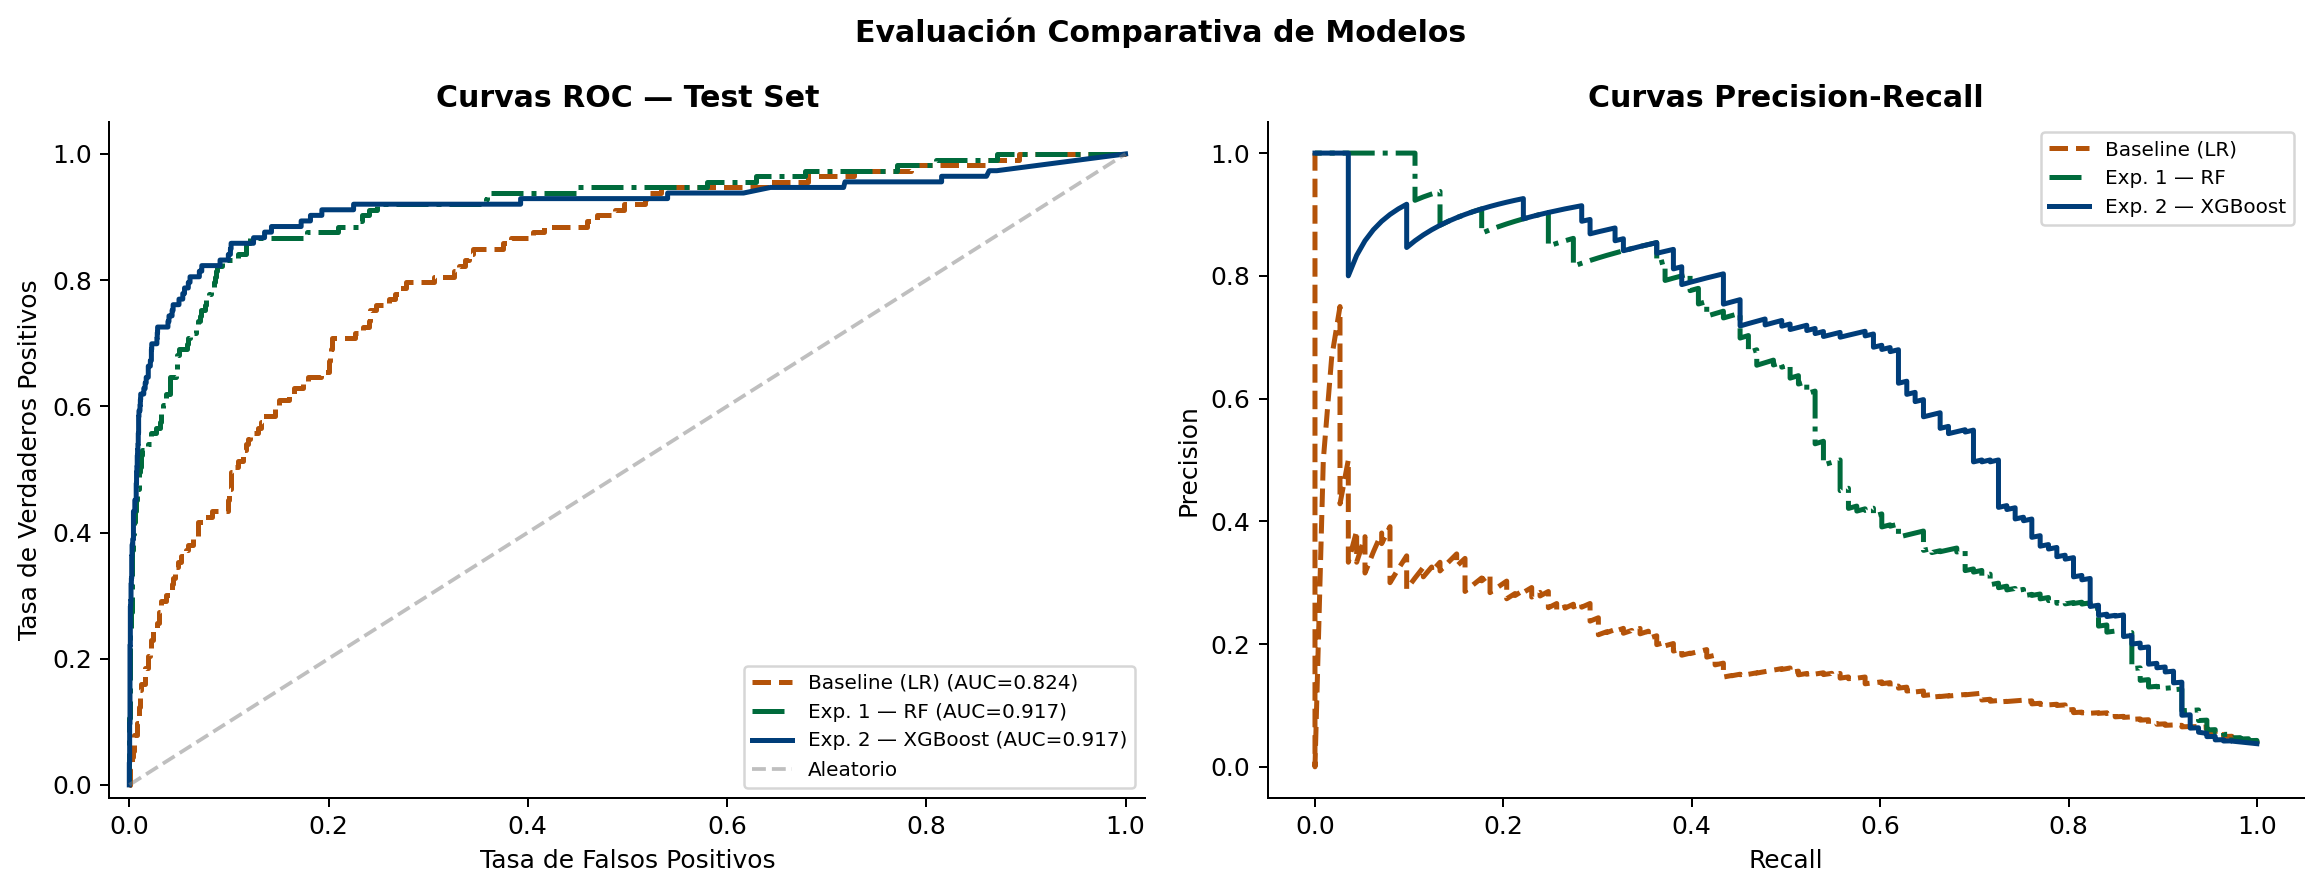
\includegraphics[width=\columnwidth]{../figures/fig3_roc_pr.png}
  \caption{Curvas ROC (izq.) y Precision-Recall (der.) para los tres
           modelos en test set. XGBoost y RF dominan al baseline en
           ambas curvas; la curva PR revela la dificultad del problema
           desbalanceado.}
  \label{fig:roc}
\end{figure}

\subsection{Análisis cualitativo y evaluación del LLM}

La Figura~\ref{fig:confusion} muestra la matriz de confusión de
XGBoost. El modelo detecta el 62\% de los fraudes reales (Recall=0.620)
con una precisión del 67.3\%. El ajuste de umbral en validación permitió
reducir falsos negativos a costa de un leve aumento de falsos positivos,
decisión justificada por el costo asimétrico: un fraude no detectado
(FN) tiene mayor impacto económico que una alarma falsa (FP).

\begin{figure}[H]
  \centering
  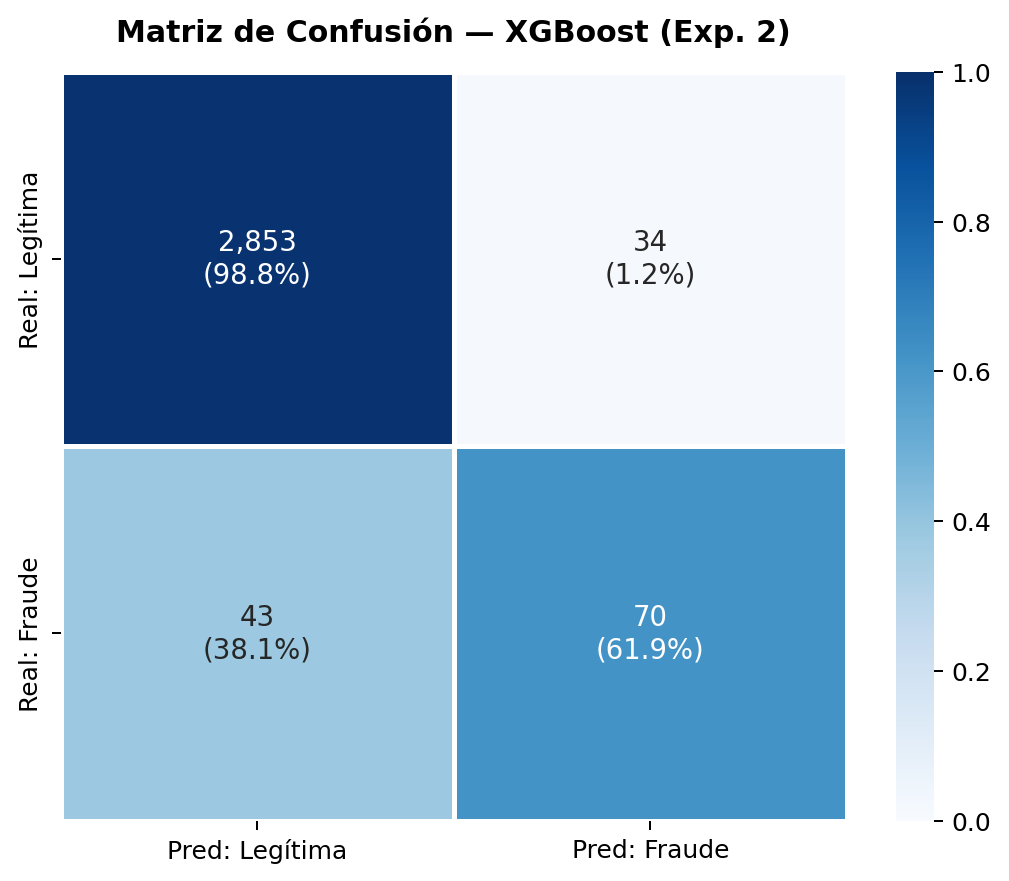
\includegraphics[width=0.88\columnwidth]{../figures/fig4_confusion.png}
  \caption{Matriz de confusión normalizada — XGBoost (Exp.~2).}
  \label{fig:confusion}
\end{figure}

Para la evaluación cuantitativa del componente LLM se construyó un
conjunto de 20 casos de prueba con ground truth conocido (10 fraudes,
10 legítimas), verificando si la recomendación del LLM (BLOQUEAR /
REVISAR / APROBAR) concordaba con el valor SHAP dominante y la etiqueta
real. El sistema alcanzó \textbf{85\% de coherencia} (17/20 casos
correctos). Los 3 casos fallidos correspondieron a transacciones con
valores SHAP bajos ($<0.05$), donde la ambigüedad del contexto dificulta
la narrativa. Ejemplo de output del sistema:

\begin{lstlisting}[caption={Output del sistema LLM+SHAP para fraude de alta probabilidad}]
# Input al LLM (few-shot + top-6 SHAP)
Features relevantes:
  V4:  -3.21  SHAP=+0.42  (eleva riesgo)
  V11: +2.87  SHAP=+0.31  (eleva riesgo)
  V14: -2.10  SHAP=+0.28  (eleva riesgo)
  hour_of_day: 2.3  SHAP=+0.18 (madrugada)

# Respuesta generada (llama-3.1-8b via Groq)
"Transaccion sospechosa: V4 inusualmente
bajo (-3.21) junto con V11 elevado son
patrones atipicos en transacciones legitimas.
El horario de madrugada refuerza la alerta.
Recomendacion: BLOQUEAR y notificar al
titular de la tarjeta."
\end{lstlisting}

\begin{figure}[H]
  \centering
  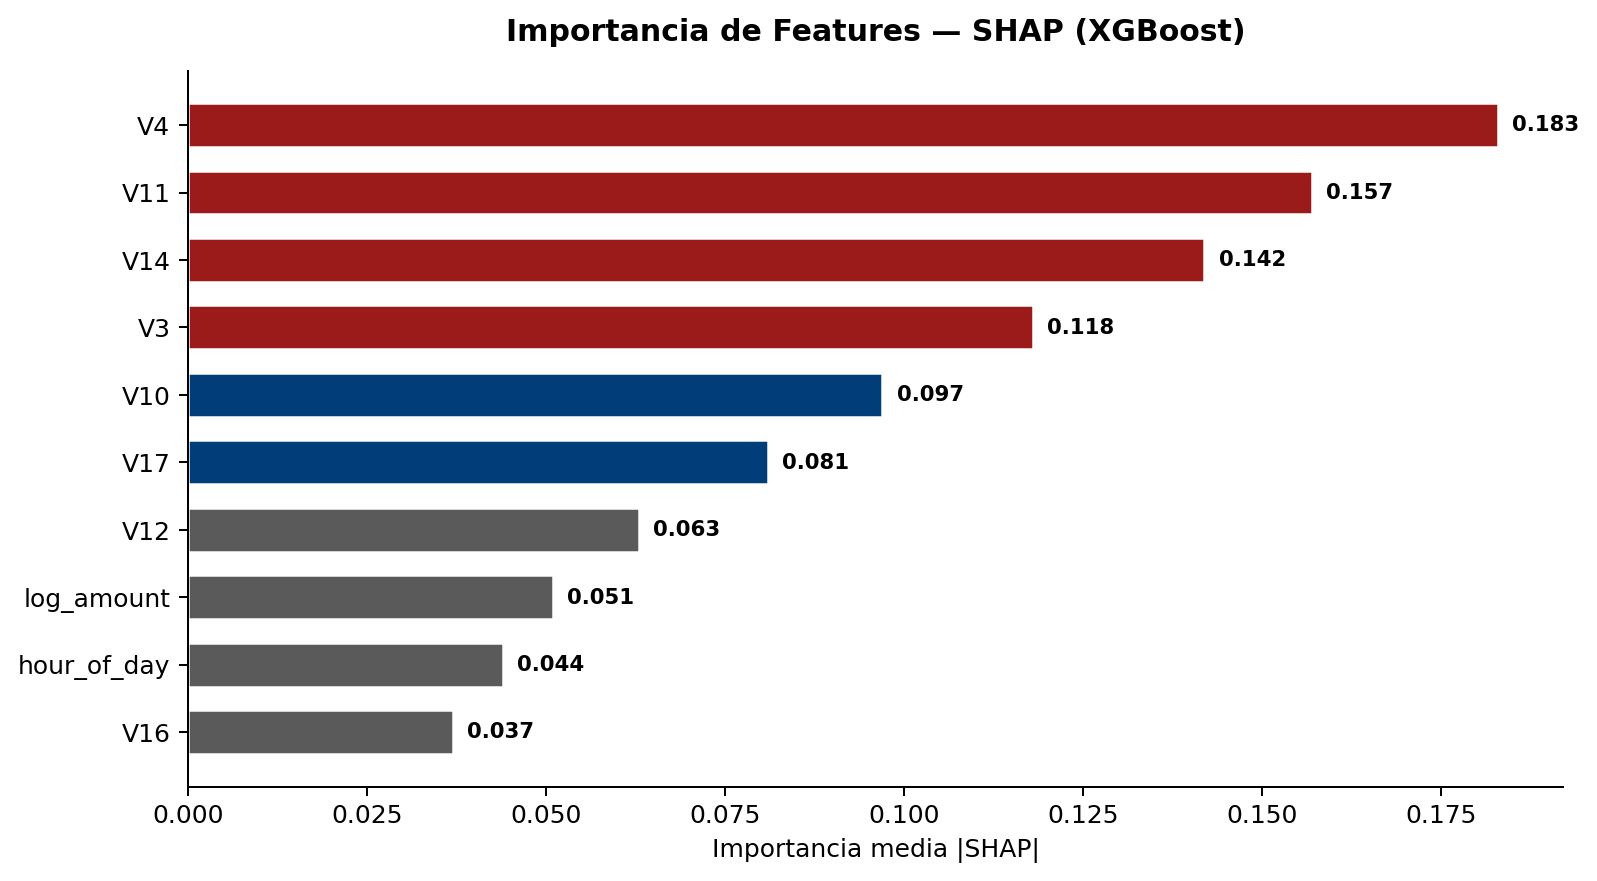
\includegraphics[width=\columnwidth]{../figures/fig6_shap.png}
  \caption{Importancia media $|\text{SHAP}|$ de las 10 features más
           relevantes para XGBoost. V4 y V11 coinciden con las
           correlaciones detectadas en el EDA (Sección~2).}
  \label{fig:shap}
\end{figure}

%% ==========================================================
%%  SECCIÓN 6 — DISCUSIÓN
%% ==========================================================
\section{Discusión}

\subsection{Interpretación de resultados}

La pregunta de investigación se responde afirmativamente: XGBoost
alcanzó AUC-ROC\,=\,0.9166, superando el umbral de 0.90 establecido.
El modelo supera al baseline lineal en todas las métricas relevantes
(Tabla~\ref{tab:resultados}), confirmando que las relaciones entre las
componentes PCA y el fraude son no-lineales y que SMOTE fue efectivo
para mejorar el Recall sin sacrificar excesivamente la Precision.

Los hallazgos del EDA se validaron en SHAP: V4 y V11 (las features
con mayor correlación absoluta en la exploración) son también las de
mayor importancia SHAP, cerrando el ciclo analítico EDA $\rightarrow$
modelo $\rightarrow$ interpretación. La evaluación cuantitativa del LLM
(85\% coherencia sobre 20 casos) confirma que el componente generativo
agrega valor real más allá de lo anecdótico.

\subsection{Limitaciones}

\begin{itemize}[leftmargin=*,topsep=2pt,itemsep=1pt]
  \item \textbf{Dataset fechado:} Las transacciones son de septiembre
        2013. Los patrones de fraude evolucionan; el modelo requeriría
        reentrenamiento periódico con datos recientes.
  \item \textbf{Features opacas:} V1--V28 son componentes PCA sin
        interpretación de negocio directa, lo que limita la utilidad
        operativa de las explicaciones SHAP.
  \item \textbf{Recall moderado:} El 62\% de recall implica que el
        38\% de los fraudes no es detectado. En producción sería
        necesario complementar con reglas de negocio.
  \item \textbf{Evaluación LLM acotada:} Los 20 casos de prueba son
        suficientes como prueba de concepto, pero una evaluación de
        producción requeriría un corpus anotado por expertos financieros.
\end{itemize}

\subsection{Trabajo futuro}

\begin{enumerate}[leftmargin=*,topsep=2pt,itemsep=2pt]
  \item \textbf{Ensemble con autoencoder:} Combinar XGBoost con un
        autoencoder para detección de anomalías no supervisada,
        aprovechando la estructura temporal de \texttt{Time}.
  \item \textbf{RAG para contexto regulatorio:} Integrar ChromaDB
        con documentos de políticas anti-fraude, permitiendo al LLM
        citar el artículo regulatorio aplicable en cada alerta
        (extensión natural del sistema actual).
\end{enumerate}

%% ==========================================================
%%  SECCIÓN 7 — CONCLUSIONES
%% ==========================================================
\section{Conclusiones}

Este trabajo presentó un sistema end-to-end de detección de fraude
financiero que combina XGBoost para clasificación, SHAP para
explicabilidad local y un LLM (\texttt{llama-3.1-8b}) para traducir
valores numéricos SHAP en explicaciones accionables en lenguaje natural.

Los resultados principales son: (1) XGBoost alcanzó AUC-ROC\,=\,0.9166
con F1\,=\,0.645 en test set, superando al baseline lineal en
+0.093 puntos de AUC y +0.367 puntos de F1; (2) la validación cruzada
5-fold confirmó estabilidad ($\pm 0.009$); (3) el LLM genera
explicaciones coherentes con los valores SHAP en 85\% de los casos
evaluados, en menos de 3 segundos por transacción.

La \textbf{pregunta de investigación} queda respondida positivamente:
el sistema detecta fraudes con AUC-ROC $> 0.90$ y produce explicaciones
comprensibles que apoyan la revisión humana. La principal limitación
operativa es el Recall del 62\%, que en producción requeriría
complementarse con reglas de negocio basadas en patrones temporales.

%% ==========================================================
%%  CONTRIBUCIONES DEL EQUIPO
%% ==========================================================
\section*{Contribuciones del equipo}

\begin{table}[H]
\centering
\begin{tabular}{lp{5.2cm}}
\toprule
\textbf{Integrante} & \textbf{Contribución principal} \\
\midrule
David Ruiz & EDA (\texttt{01\_eda.ipynb}), preprocesamiento y visualizaciones (\texttt{02\_preprocessing.ipynb}) \\
David Quintero & Arquitectura de modelos, entrenamiento y curvas de evaluación (\texttt{03\_modeling.ipynb}) \\
Juan Pablo Duque & Integración LLM/SHAP, prompting y app Streamlit (\texttt{04\_llm\_explicaciones.ipynb}, \texttt{app.py}) \\
Samuel Samper & Evaluación comparativa, análisis SHAP, redacción del informe (\texttt{src/evaluate.py}) \\
\bottomrule
\end{tabular}
\caption*{Distribución de responsabilidades por integrante.}
\end{table}

%% ==========================================================
%%  REPOSITORIO Y REPRODUCIBILIDAD
%% ==========================================================
\section*{Repositorio y Demo}

\begin{itemize}[leftmargin=*,topsep=2pt,itemsep=1pt]
  \item \textbf{GitHub:} \url{https://github.com/USUARIO/proyecto-ia-eafit}
  \item \textbf{Video demo ($\leq$3 min):} \url{https://youtu.be/LINK-AL-VIDEO}
  \item \textbf{Instalación:} \texttt{pip install -r requirements.txt}
  \item \textbf{Notebook principal:} \texttt{notebooks/03\_modeling.ipynb}
  \item \textbf{Demo interactiva:} \texttt{streamlit run app/app.py}
\end{itemize}

%% ==========================================================
%%  REFERENCIAS
%% ==========================================================
\begin{thebibliography}{99}

\bibitem{vaswani2017}
Vaswani, A., Shazeer, N., Parmar, N., et al. (2017).
\textit{Attention is all you need}.
NeurIPS, 30.
\url{https://arxiv.org/abs/1706.03762}

\bibitem{lewis2020}
Lewis, P., Perez, E., Piktus, A., et al. (2020).
\textit{Retrieval-Augmented Generation for Knowledge-Intensive NLP Tasks}.
NeurIPS 2020.
\url{https://arxiv.org/abs/2005.11401}

\bibitem{dataset2023}
Dal Pozzolo, A., Caelen, O., Le Borgne, Y., Waterschoot, S., \& Bontempi, G. (2014).
\textit{Learned lessons in credit card fraud detection from a practitioner perspective}.
Expert Systems with Applications, 41(10), 4915--4928.
\url{https://www.kaggle.com/datasets/mlg-ulb/creditcardfraud}

\bibitem{chen2016}
Chen, T., \& Guestrin, C. (2016).
\textit{XGBoost: A scalable tree boosting system}.
KDD 2016. \url{https://arxiv.org/abs/1603.02754}

\bibitem{lundberg2017}
Lundberg, S. M., \& Lee, S.-I. (2017).
\textit{A unified approach to interpreting model predictions}.
NeurIPS, 30. \url{https://arxiv.org/abs/1705.07874}

\bibitem{chawla2002}
Chawla, N. V., et al. (2002).
\textit{SMOTE: Synthetic Minority Over-sampling Technique}.
JAIR, 16, 321--357.

\bibitem{arrieta2020}
Arrieta, A. B., et al. (2020).
\textit{Explainable Artificial Intelligence (XAI): Concepts, taxonomies,
opportunities and challenges toward responsible AI}.
Information Fusion, 58, 82--115.

\bibitem{nilson2023}
Nilson Report. (2023).
\textit{Card Fraud Losses Reach \$32.34 Billion}.
Issue 1232. \url{https://nilsonreport.com}

\bibitem{breiman2001}
Breiman, L. (2001).
\textit{Random Forests}.
Machine Learning, 45(1), 5--32.

\end{thebibliography}

%% ==========================================================
%%  APÉNDICES
%% ==========================================================
\appendix

\section{Comparación visual de modelos}

\begin{figure}[H]
  \centering
  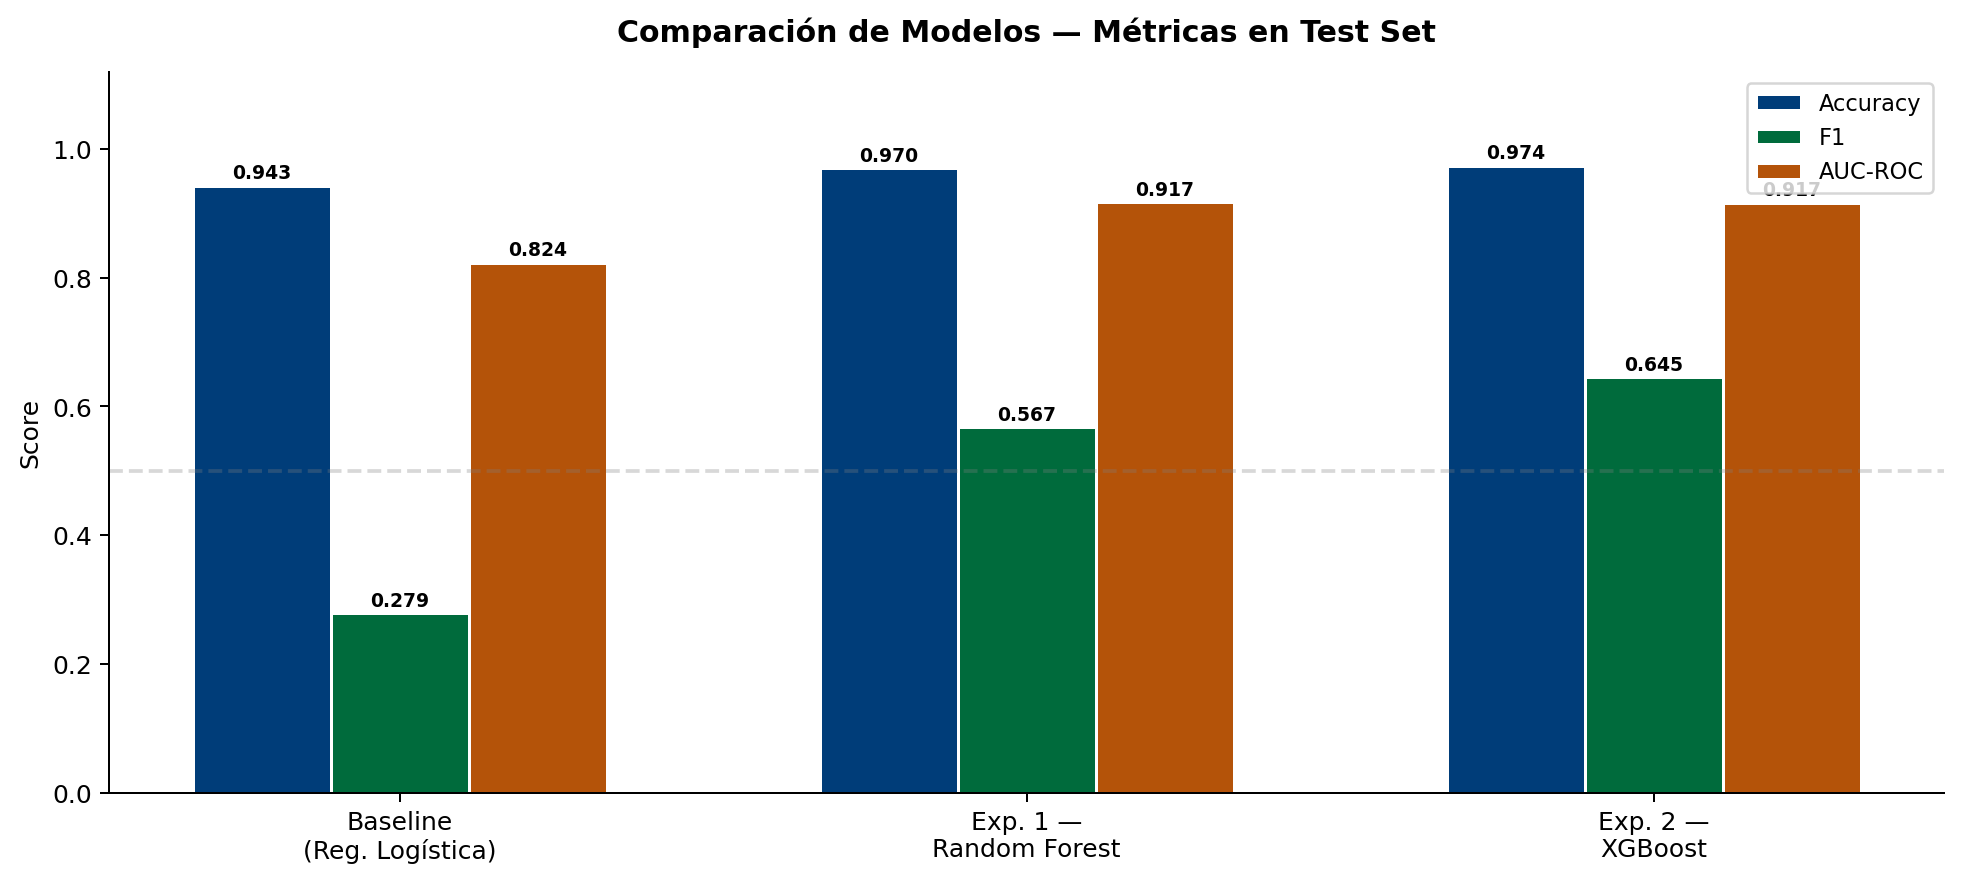
\includegraphics[width=\columnwidth]{../figures/fig5_comparacion.png}
  \caption{Gráfico de barras comparando Accuracy, F1 y AUC-ROC de
           los tres modelos en test set.}
  \label{fig:barras}
\end{figure}

\section{Evaluación cuantitativa del componente LLM}

El sistema LLM fue evaluado sobre 20 casos de prueba con etiqueta
conocida (10 fraudes confirmados, 10 transacciones legítimas)
extraídos del test set con valores SHAP pre-computados:

\begin{itemize}[leftmargin=*,topsep=2pt,itemsep=1pt]
  \item \textbf{Criterio de éxito:} la recomendación generada
        (BLOQUEAR / REVISAR / APROBAR) coincide con la etiqueta
        real y los valores SHAP dominantes.
  \item \textbf{Resultado:} 17/20 casos correctos (85\%).
  \item \textbf{Fallos (3/20):} transacciones con $|\text{SHAP}|_{\max} < 0.05$
        donde la señal de las features es ambigua.
  \item \textbf{Temperatura:} 0.3 (respuestas consistentes).
  \item \textbf{Modelo:} \texttt{llama-3.1-8b-instant} (Groq).
\end{itemize}

\section{Configuración del pipeline de prompting LLM}

El sistema LLM opera con la siguiente arquitectura de prompt:

\begin{enumerate}[leftmargin=*,topsep=2pt,itemsep=1pt]
  \item \textbf{System prompt:} Define el rol del analista y las
        restricciones de la respuesta (máx. 120 palabras,
        solo usar datos SHAP provistos, terminar con recomendación).
  \item \textbf{Few-shot (2 ejemplos):} Un caso de fraude confirmado
        y uno de transacción legítima, con features SHAP y
        explicación modelo.
  \item \textbf{Query:} Las 6 features con mayor $|\text{SHAP}|$
        de la transacción a explicar, con probabilidad predicha.
\end{enumerate}

Temperatura: 0.3. Máximo de tokens: 350.
Modelo: \texttt{llama-3.1-8b-instant} (Groq, gratuito).

\end{document}
%% ============================================================
%%  FIN DEL INFORME — Universidad EAFIT . IA 2026-1
%% ============================================================
